\documentclass[12pt]{article}

\usepackage{polski}
\usepackage[utf8]{inputenc}
\usepackage[T1]{fontenc}
%\usepackage{indentfirst}
\usepackage{amsfonts}
\usepackage{graphicx}
\usepackage{caption}
\usepackage{multirow}
\usepackage{booktabs}
\usepackage{amssymb}
\usepackage[top=2cm, bottom=2cm, left=3cm, right=3cm]{geometry}
\usepackage{mathrsfs}
\usepackage{tikz}
\usepackage{pgfplots}
%\pagestyle{empty}
\usepackage{listings}
\usepackage{titlesec}
\usepackage{hyperref}
\usepackage{graphicx}
\usepackage{subfig}
\usepackage{natbib}
\usepackage{rotating}
\usepackage{float}

\title{\textbf{Sprawozdanie - stacja do wykrywania wyładowań atmosferycznych}\\KN EKSA}
\author{Michał Wieczorek {226284}\\ Amadeusz Wach {226379}\\ Rafał Różycki {226367} \\ Mateusz Otto {226312}}
\date{\today}

\begin{document}
\maketitle
\newpage

\section{Opis projektu}
Celem projektu jest konstrukcja niskobudżetowego uniwersalnego odbiornika fal krótkich o zakresie częstotliwości 3 kHz - 300 kHz. Wyładowanie atmosferyczne generuje fale elektromagnetyczne w bardzo szerokim zakresie częstotliwości. Są to impulsy, które mogą zostać odebrane ponad 1000 km od wystąpienia wyładowania. Szczegółowy teoretyczny opis zjawiska można znaleźć np. na Wikipedii. Dla częstotliwości niższych niż 100 kHz impulsy wyraźnie wybijają się ponad szum atmosferyczny, co pozwala z łatwością odebrać sygnał. Odbiornik będzie posiadać dwa wejścia na anteny ferrytowe typu H-field, co pozwoli określić przybliżoną odległość i kierunek odebranego sygnału. Anteny zostaną skonstruowane przez wykonawców projektu, ich parametry zostaną eksperymentalnie wyznaczone. Po pomyślnym zainstalowaniu odbiornika następnym krokiem będzie konstrukcja kilku następnych, co pozwoli na dokładniejsze określenie lokalizacji wystąpienia wyładowania za pomocą porównań czasów odebrania sygnału (Time of arrival method). Dane z odbiornika będą przesyłane na serwer w celu ich analizy. Projekt zakłada ukończenie prac nad jednym odbiornikiem i uruchomienie go przed końcem roku 2017. Jednym z założeń jest łatwe wprowadzanie zmian i dodatkowych modułów do odbiornika tak, aby jego użytkownicy mogli dalej go rozwijać oraz mieli możliwość prowadzenia badań. Planowane jest udostępnienie ukończonej stacji do użytku jako projekt wykonany w kole naukowym.

\section{Zrealizowane zadania i testy}
0. Symulacja wzmacniacza w programie LTspice. Charakterystyka częstotliwościowa.\\
\begin{figure}[H]
\begin{center}
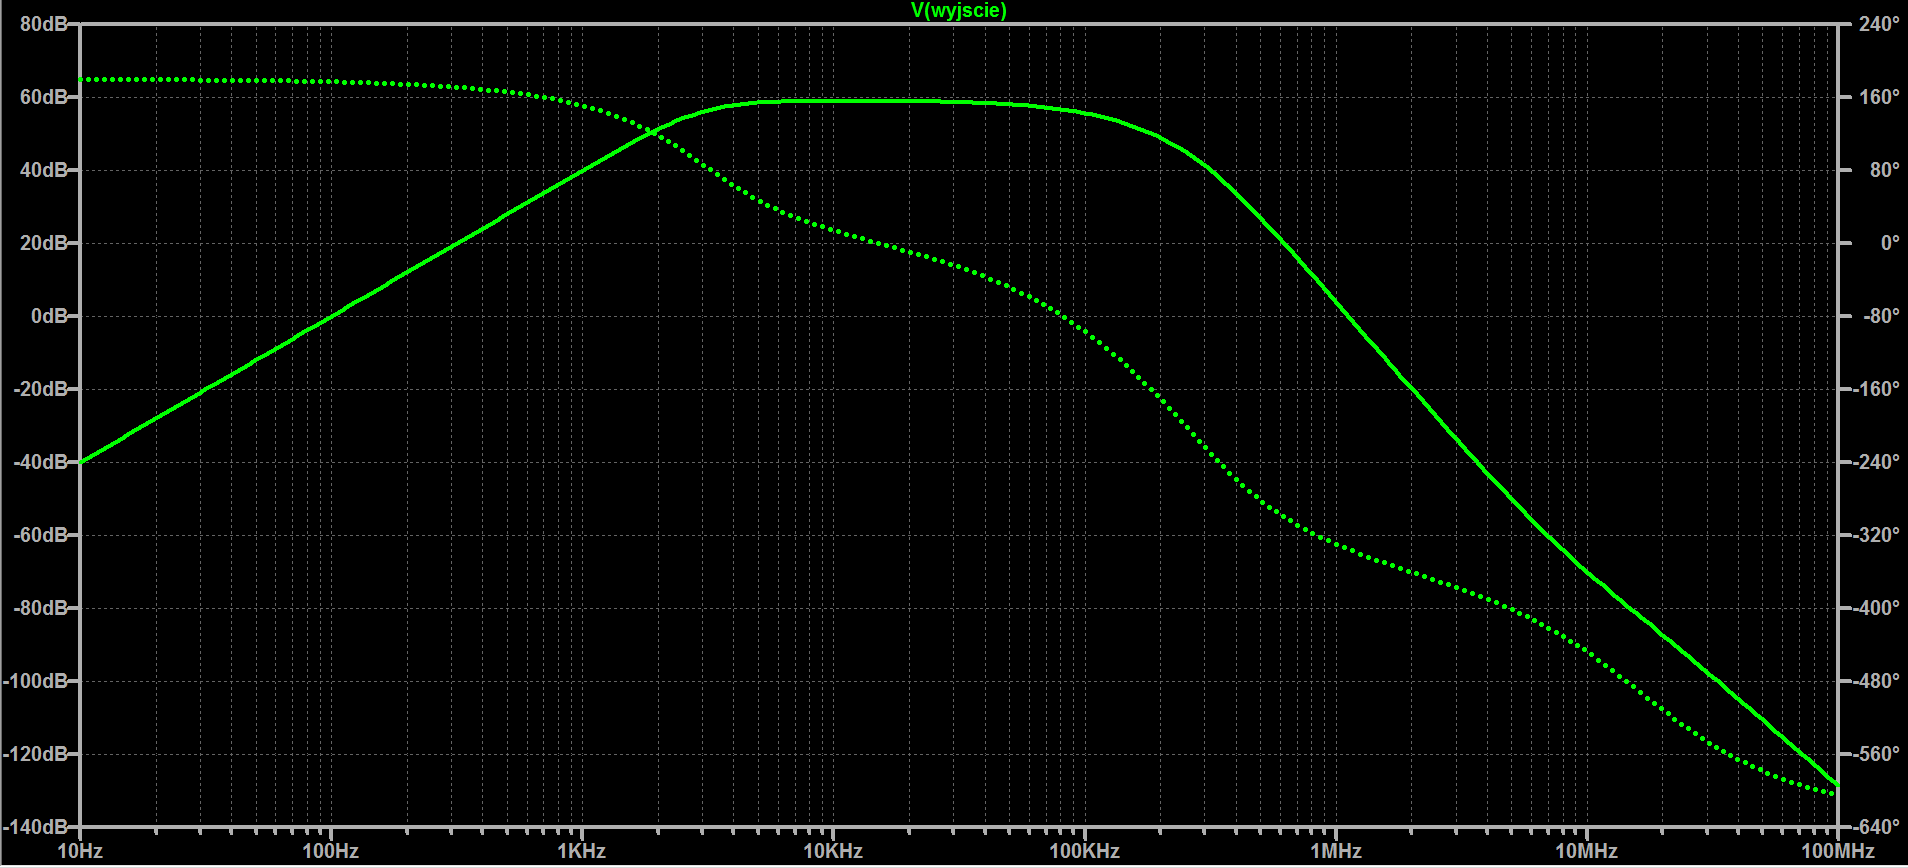
\includegraphics[width=1\textwidth]{figures/ampl_faz.png}
\caption{Charakterystyka amplitudowa i fazowa układu}
\end{center}
\end{figure}
1. Prototyp wzmacniacza na płytce prototypowej\\
2. Budowa anten kierunkowych\\
3. Testowanie czujnika [generator + oscyloskop]\\
4. Polutowanie prototypowego wzmacniacza z poprawkami\\
\begin{figure}[H]
\begin{center}
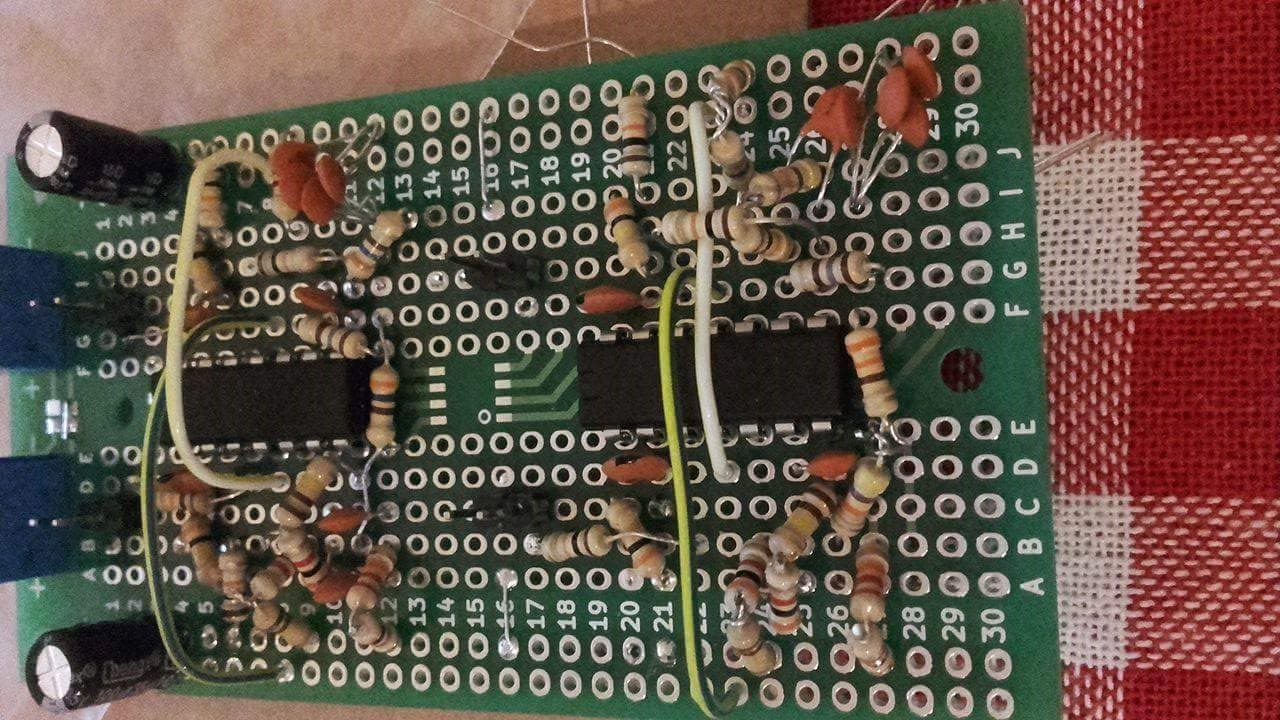
\includegraphics[width=0.95\textwidth]{figures/plytka.png}
\caption{Będzie inne zdjęcie}
\end{center}
\end{figure}
5. Testy czujnika [przesyłanie sygnału przez indukcję]\\
6. Testy czujnika w pobliżu burzy, reakcja na wyładowania\\
7. Próbkowanie sygnały analogowego. Płytka nucleo, schemat + testy (STMStudio).\\
\begin{figure}[H]
\begin{center}
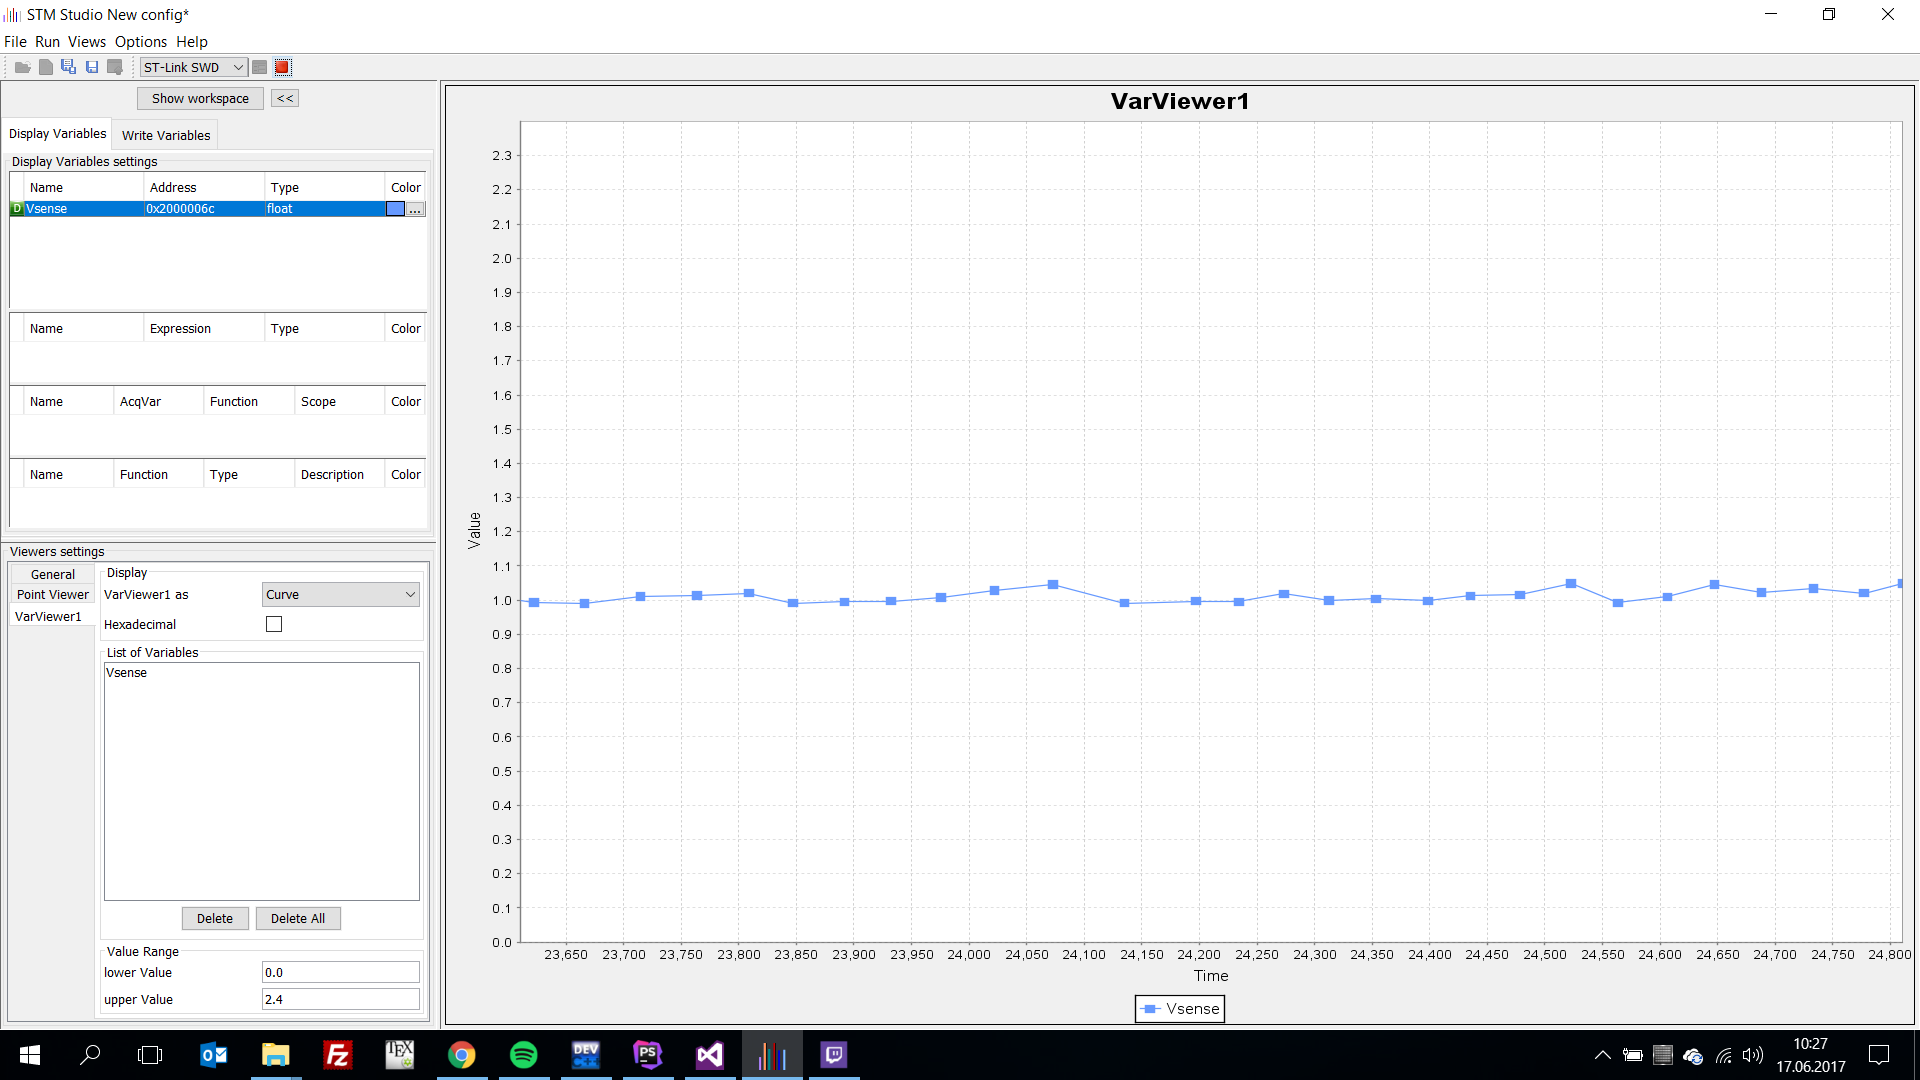
\includegraphics[width=0.95\textwidth]{figures/stmstudio.png}
\caption{STMStudio - obserwacja napięcia na wyjściu wzmacniacza}
\end{center}
\end{figure}

\section{Kontynuacja projektu?}
Co zamierzamy zrobić w najbliższym czasie.

\end{document}